\documentclass[English,c,% 't' (resp. 'c') places text vertically at top/center of each slide
% PDF settings
hyperref={%
    pdftitle={FISA-DE2 JavaDoc},%
    pdfauthor={Muller, Gravier, Laforest, Subercaze},%
    pdfsubject={JavaDoc},%
    pdfkeywords={Java, JavaDoc},%
    colorlinks=true,%
    urlcolor=blue,%
    linkcolor=%
    },%
% To load many pre-defined color names
xcolor={pdftex,svgnames} % dvipsnames, dvipsnames*, svgnames, svgnames*, x11names,
]{beamer}

\usetheme{Copenhagen}
%\setbeamertemplate{footline}[page number]
%\setbeamertemplate{frametitle}[default][center]
% To remove the navigation symbols from the bottom of slides:

% Remove navigation bar
\setbeamertemplate{navigation symbols}{}
% Remove outline at top
\setbeamertemplate{headline}{}

% Put text more on top of each slide for all slides
\addtobeamertemplate{frametitle}{}{\vspace*{-.7em}}

% Correct French/English indentation and splitting of words
\usepackage{babel}

% Correct management of accentuated chars in input file
\usepackage[utf8]{inputenc}

% Correct font for the generation of docs with accentuated chars
\usepackage[T1]{fontenc}      % Can handle hyphenation of words with accented characters
%%\usepackage[OT1]{fontenc}   % Might generated bad looking PDFs

% Insertion of images generated by external tools
\usepackage{graphicx}
% To generate pretty & scalable images directly in LaTeX
\usepackage{tikz}

% To print numbers correctly
\usepackage{numprint}

\usepackage[absolute,overlay]{textpos}

\usepackage{fourier}

\setbeamercovered{transparent}
\setbeamercovered{invisible}

\AtBeginSection[]
{
   \begin{frame}
       \frametitle{Plan}
       \tableofcontents[currentsection]
   \end{frame}
}

\usepackage{url,manfnt}


% To be able to insert code listing
\usepackage{listings}

\definecolor{dkgreen}{rgb}{0,0.6,0}
\definecolor{gray}{rgb}{0.5,0.5,0.5}
\definecolor{mauve}{rgb}{0.58,0,0.82}

\lstset{frame=none,
  language=Java,
  aboveskip=1mm,
  belowskip=1mm,
  showstringspaces=false,
  columns=flexible,
  basicstyle={\tiny \ttfamily},
  numbers=left,
  numberstyle=\tiny\color{gray},
  keywordstyle=\color{blue},
  commentstyle=\color{dkgreen},
  stringstyle=\color{mauve},
  breaklines=true,
  breakatwhitespace=true,
  tabsize=2
}
\definecolor{algoTitle}{rgb}{0.84,0.83,0.94}

\usepackage{caption}
\DeclareCaptionFont{white}{\color{white}}
\DeclareCaptionFormat{listing}{\colorbox{algoTitle}{\parbox{\textwidth}{\bfseries #1#2 #3}}}
\captionsetup[lstlisting]{format=listing,labelfont=white,textfont=white}

\title[JavaDoc]{JavaDoc}
\logo{
\includegraphics[width=1cm]{images00/logo_tse.png}}
\author[Guillaume MULLER]{
  Guillaume \textsc{Muller}\\
  {\scriptsize \textit{based on work from:} \\
    Ch. \textsc{Gravier}, F. \textsc{Laforest}, J. \textsc{Subercaze}}
}
\institute[TSE/UJM]{
  Télécom Saint-\'{E}tienne\\
  \medskip
  {\url{{pénom.nom}@univ-st-etienne.fr}}
}
\date[09/14/2020]{14~September~2020}

\begin{document}

%%%%%%%%%%%%%%%%%%%%%%%%%%%%%%%%%%%%%%%%%%%%%%%%%%%%%%%%%%%%%%%%%%%%%%
\begin{frame}
  \maketitle
\end{frame}

\section{Documentation -- Javadoc}

%%%%%%%%%%%%%%%%%%%%%%%%%%%%%%%%%%%%%%%%%%%%%%%%%%%%%%%%%%%%%%%%%%%%%%
\begin{frame}{Javadoc tool}
\begin{itemize}
  \item Comments are introduced by:\\
  \texttt{/* \ldots{} */} (multi-line) or \texttt{// \ldots{}} (mono-line)
  \item Class/Attribute/Method \textbf{documentation} is introduced by:\\
  \texttt{/** */}
  \item The documentation can contain HTML tags (\texttt{<b>}, \texttt{<code>}\ldots{})
  \item Documentation comments are split in two parts:
  {\small
    \begin{itemize}
      \item A description in natural language,
      \item A set of tags to identify specific/important information (\texttt{@Author}, \texttt{@Result}\ldots{}).
    \end{itemize}
  }
  \item JDK provides a tool for generating the documentation: \texttt{javadoc} (\textbf{java doc}umentation);
\end{itemize}
\end{frame}



%%%%%%%%%%%%%%%%%%%%%%%%%%%%%%%%%%%%%%%%%%%%%%%%%%%%%%%%%%%%%%%%%%%%%%
\begin{frame}[fragile]{Example\footnote{\url{http://tinyurl.com/2vrongv}}}
\vspace{-1.3em}
{\small
  \begin{lstlisting}[escapechar=\%,label=intex,caption=JavadocExample.java,basicstyle=\footnotesize]
/**
* <p>Returns an Image object that can then be painted on the screen.</p>
* <p>The url argument must specify an absolute {@link URL}.
* The name argument is a specifier that is relative to the url argument.</p>
* @param  url    An absolute URL of the image
* @param  name   The image location relative to the url
* @return        The image at the specified URL
* @see           Image
*/
 public Image getImage(URL url, String name) {
   // do something
   return null;
}
\end{lstlisting}
}
\end{frame}


%%%%%%%%%%%%%%%%%%%%%%%%%%%%%%%%%%%%%%%%%%%%%%%%%%%%%%%%%%%%%%%%%%%%%%
\begin{frame}{Result after calling \texttt{javadoc}: navigable HTML}
  \begin{figure}
    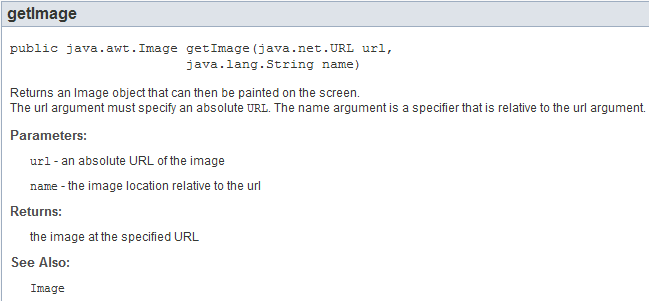
\includegraphics[width=1\textwidth]{./images01/javadoc.png}
  \end{figure}
\end{frame}


%%%%%%%%%%%%%%%%%%%%%%%%%%%%%%%%%%%%%%%%%%%%%%%%%%%%%%%%%%%%%%%%%%%%%%
\begin{frame}{Possible Tags\footnote{\url{http://tinyurl.com/8uvaclp}}}
  \begin{itemize}
    \item \texttt{@author} (classes and interfaces only, required)
    \item \texttt{@version} (classes and interfaces only, required)
    \item \texttt{@param} (methods and constructors only)
    \item \texttt{@return} (methods only)
    \item \texttt{@exception} (@throws is a synonym added in Javadoc 1.2)
    \item \texttt{@see}
    \item \texttt{@since}
    \item \texttt{@serial} (or @serialField or @serialData)
    \item \texttt{@deprecated} (see How and When To Deprecate APIs)
  \end{itemize}
\end{frame}

\end{document}
